Consider three well-known ports that appear in both source and destination traffic in Table 2: 21, 161 and 514.

\begin{figure}[!htb]
	\centering
	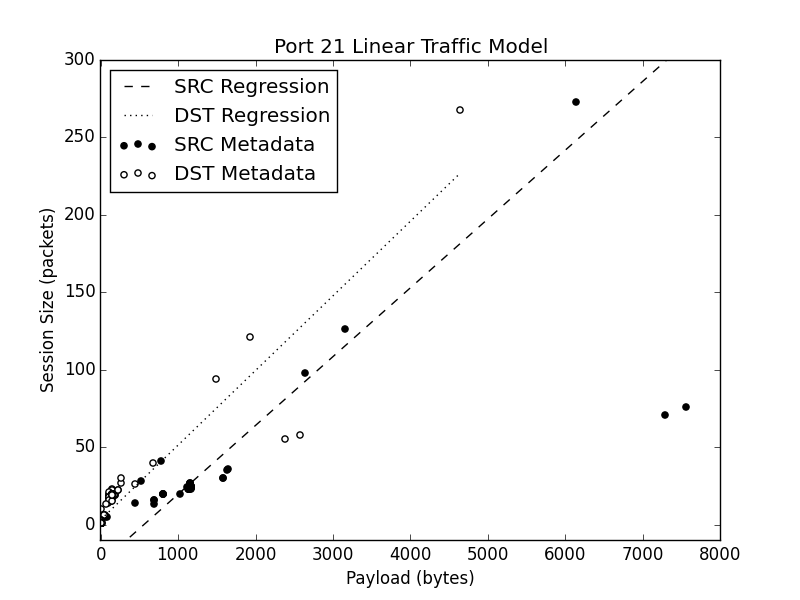
\includegraphics[width=9cm]{paperplots/21.png}
	\caption{FTP Traffic Model (1 min Snapshot)}
	\label{fig:21}
\end{figure}

Port 21, associated with File Transfer Protocol (FTP), has higher classification performance as a source (when the server is responding) versus the destination (when the client is sending). This is due to the nature of FTP, where server responses (port 21 as the source) are short and convey connection state information back to the client. Table \ref{tab:direction} has been provided for illustrative purposes of directional semantics. By nature, we would expect this traffic to have generalizable linear characteristics simply due to the fact a machine is the source of this traffic, and we believe this holds up in our analysis (see Figure \ref{fig:21}).

\begin{figure}[!htb]
	\centering
	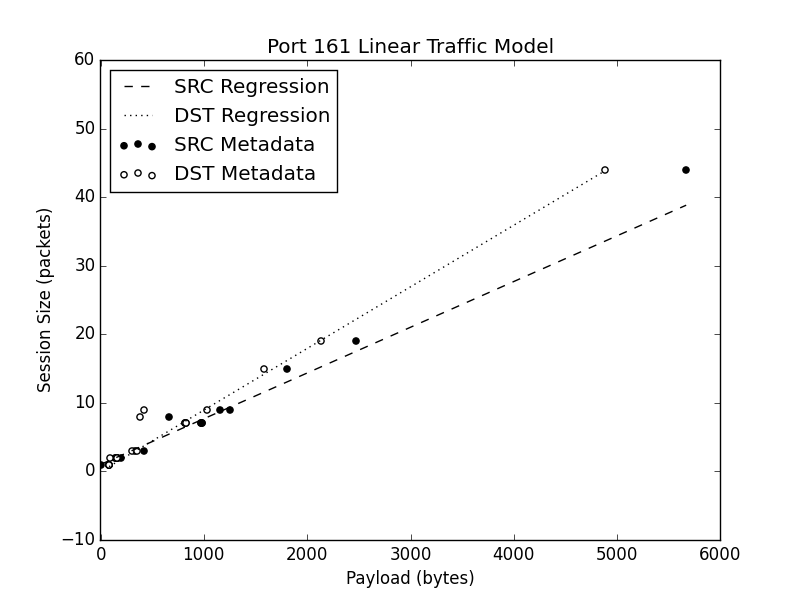
\includegraphics[width=9cm]{paperplots/161.png}
	\caption{SNMP Traffic Model (1 min Snapshot)}
	\label{fig:161}
\end{figure}

\begin{figure}[!htb]
	\centering
	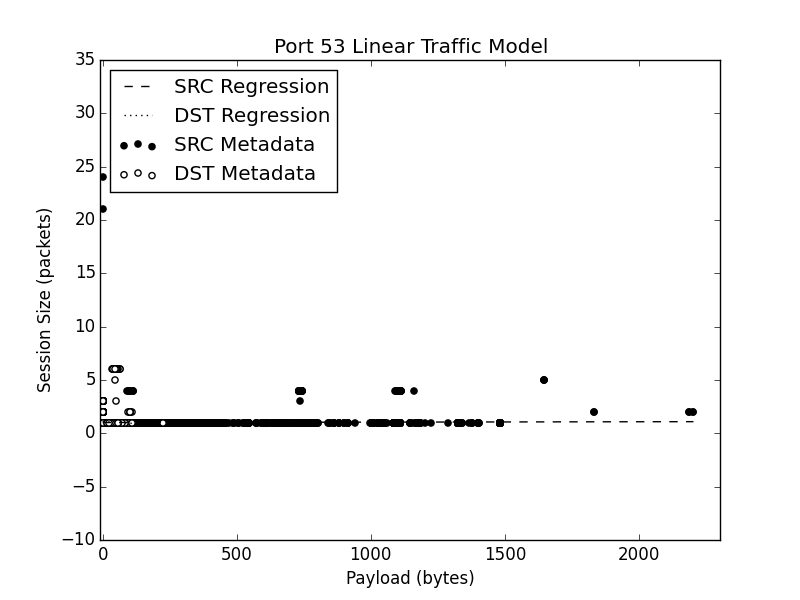
\includegraphics[width=9cm]{paperplots/53.png}
	\caption{DNS Traffic Model (1 min Snapshot)}
	\label{fig:53}
\end{figure}

Similarly, the same can be said of Port 161 (seen in Figure \ref{fig:161}), associated with Simple Network Management Protocol (SNMP) facilitating management of devices on a network by collecting data as well as changing device configuration information, as well as Domain Name Service (DNS) traffic on Port 53 (Figure \ref{fig:53}) resolving domain IP addresses. Given the preponderance of machine-generated traffic, behaving semi-deterministically, there lies a strong possibility for performing such network characterization to identify malicious traffic attempting to masquerade in this linear space \cite{7033254}.





However nondeterministic, user-based traffic is not necessarily out of reach from this effort. Figure \ref{fig:80} and \ref{fig:443} represent a one minute snapshot of unencrypted web traffic and both encrypted web and VPN traffic respectively. Although the intermediate model looks promising, the performance of Port 80 was 18.65\% on source traffic and 0.95\% on destination traffic, considerably lower than the top 10 in Table \ref{t:accuracy}. The disparity is due to the scale of the session payloads and the volume of traffic. Overall, web traffic (both encrypted and unencrypted) is a preponderance of the data, 99\% of which falling between 0-93kb in size and 1-71 packets in length. While this poses problems in terms of linear differentiability, we believe this could be overcome using hierarchical approaches.

Performing linear regression by applying the same technique on unique IP pairs within port 80 and 443 traffic adds another layer of behavioral characterization that can be captured. As an illustrative example, unencrypted UDP traffic originating from \texttt{espn.com} comprising of streaming video content would have a significantly different profile and patten to that of unencrypted TCP traffic from \texttt{bbc.com}. Likewise, encrypted UDP video traffic from \texttt{youtube.com} would have a different linear footprint than that of a standard search on \texttt{google.com}.

\begin{figure}[!htb]
	\centering
	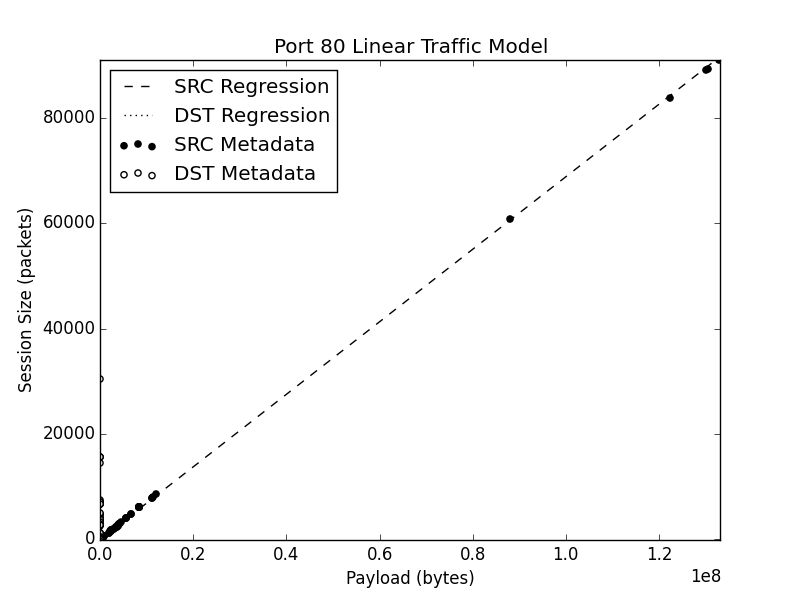
\includegraphics[width=9cm]{paperplots/80.png}
	\caption{Unencrypted Web Traffic Model (1 min Snapshot)}
	\label{fig:80}
\end{figure}

\begin{figure}[!htb]
	\centering
	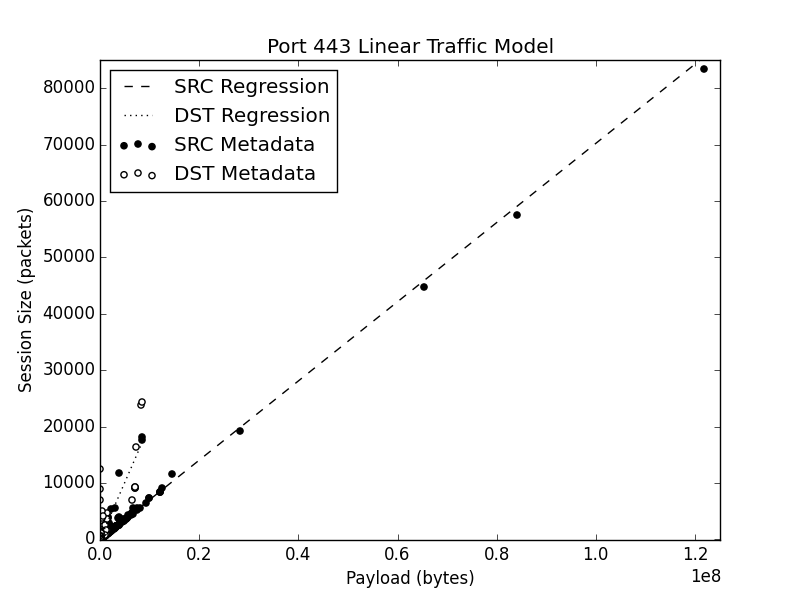
\includegraphics[width=9cm]{paperplots/443.png}
	\caption{Encrypted Web/VPN Traffic Model (1 min Snapshot)}
	\label{fig:443}
\end{figure}

